% -*-coding: utf-8 -*-
%%%%%%%%%%%%%%%%%%%%%%%%%%%%%%%%%%%%%%%%%
% Plain Cover Letter
% LaTeX Template
% Version 1.0 (28/5/13)
%
% This template has been downloaded from:
% http://www.LaTeXTemplates.com
%
% Original author:
% Rensselaer Polytechnic Institute 
% http://www.rpi.edu/dept/arc/training/latex/resumes/
%
% License:
% CC BY-NC-SA 3.0 (http://creativecommons.org/licenses/by-nc-sa/3.0/)
%
%%%%%%%%%%%%%%%%%%%%%%%%%%%%%e%%%%%%%%%%%%

%----------------------------------------------------------------------------------------
%	PACKAGES AND OTHER DOCUMENT CONFIGURATIONS
%----------------------------------------------------------------------------------------

\documentclass[11pt]{article} % Default font size of the document, change to 10pt to fit more text
\usepackage[utf8]{inputenc}
\usepackage{newcent} % Default font is the New Century Schoolbook PostScript font 
%\usepackage{helvet} % Uncomment this (while commenting the above line) to use the Helvetica font
\usepackage{pdfpages}
\usepackage{graphicx}
% Margins
\topmargin=-1in % Moves the top of the document 1 inch above the default
\textheight=8.5in % Total height of the text on the page before text goes on to the next page, this can be increased in a longer letter
\oddsidemargin=-10pt % Position of the left margin, can be negative or positive if you want more or less room
\textwidth=6.5in % Total width of the text, increase this if the left margin was decreased and vice-versa

%\let\raggedleft\raggedright % Pushes the date (at the top) to the left, comment this line to have the date on the right

\begin{document}

%----------------------------------------------------------------------------------------
%	ADDRESSEE SECTION
%----------------------------------------------------------------------------------------

%\name{Santiago Bragagnolo}
\date{}%29 Juin 2015}

\author{Santiago Bragagnolo} % Your name for the signature at the bottom

%----------------------------------------------------------------------------------------
%	LETTER CONTENT SECTION
%----------------------------------------------------------------------------------------
%29 Juin 2015

\title{Objet: Inscription Ecole Doctorale }
\maketitle



 Ici je rajoute successivement les documents nécessaires pour la ouverture d'une compte ADUM et la posterior inscription a l'Ecole Doctorale SPI.
 La table suivant montre la disposition de chaque document dans ce PDF.


\tableofcontents

\section{Lettre de motivation}
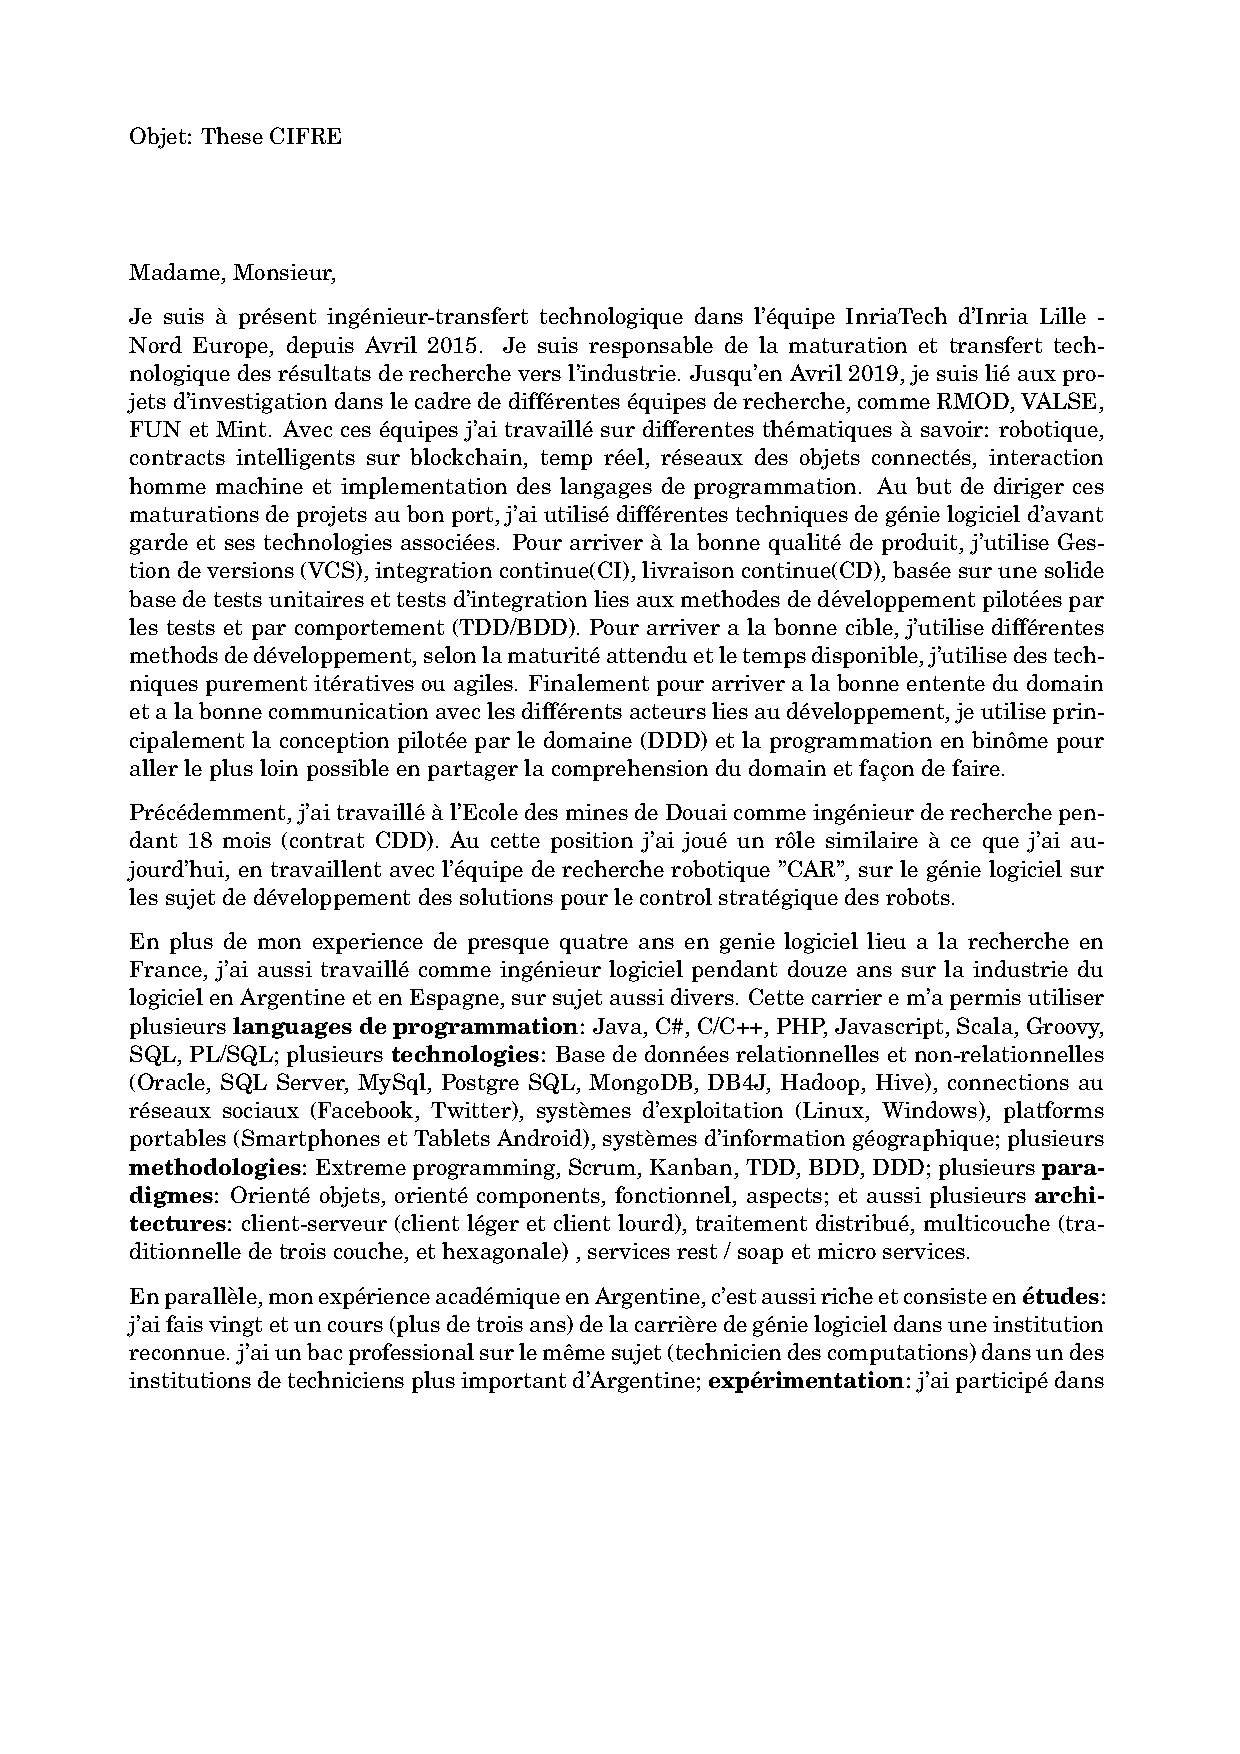
\includepdf[pages=-]{docs/Doc1-Motivation.pdf}
 
\section{Curriculum Vitae}
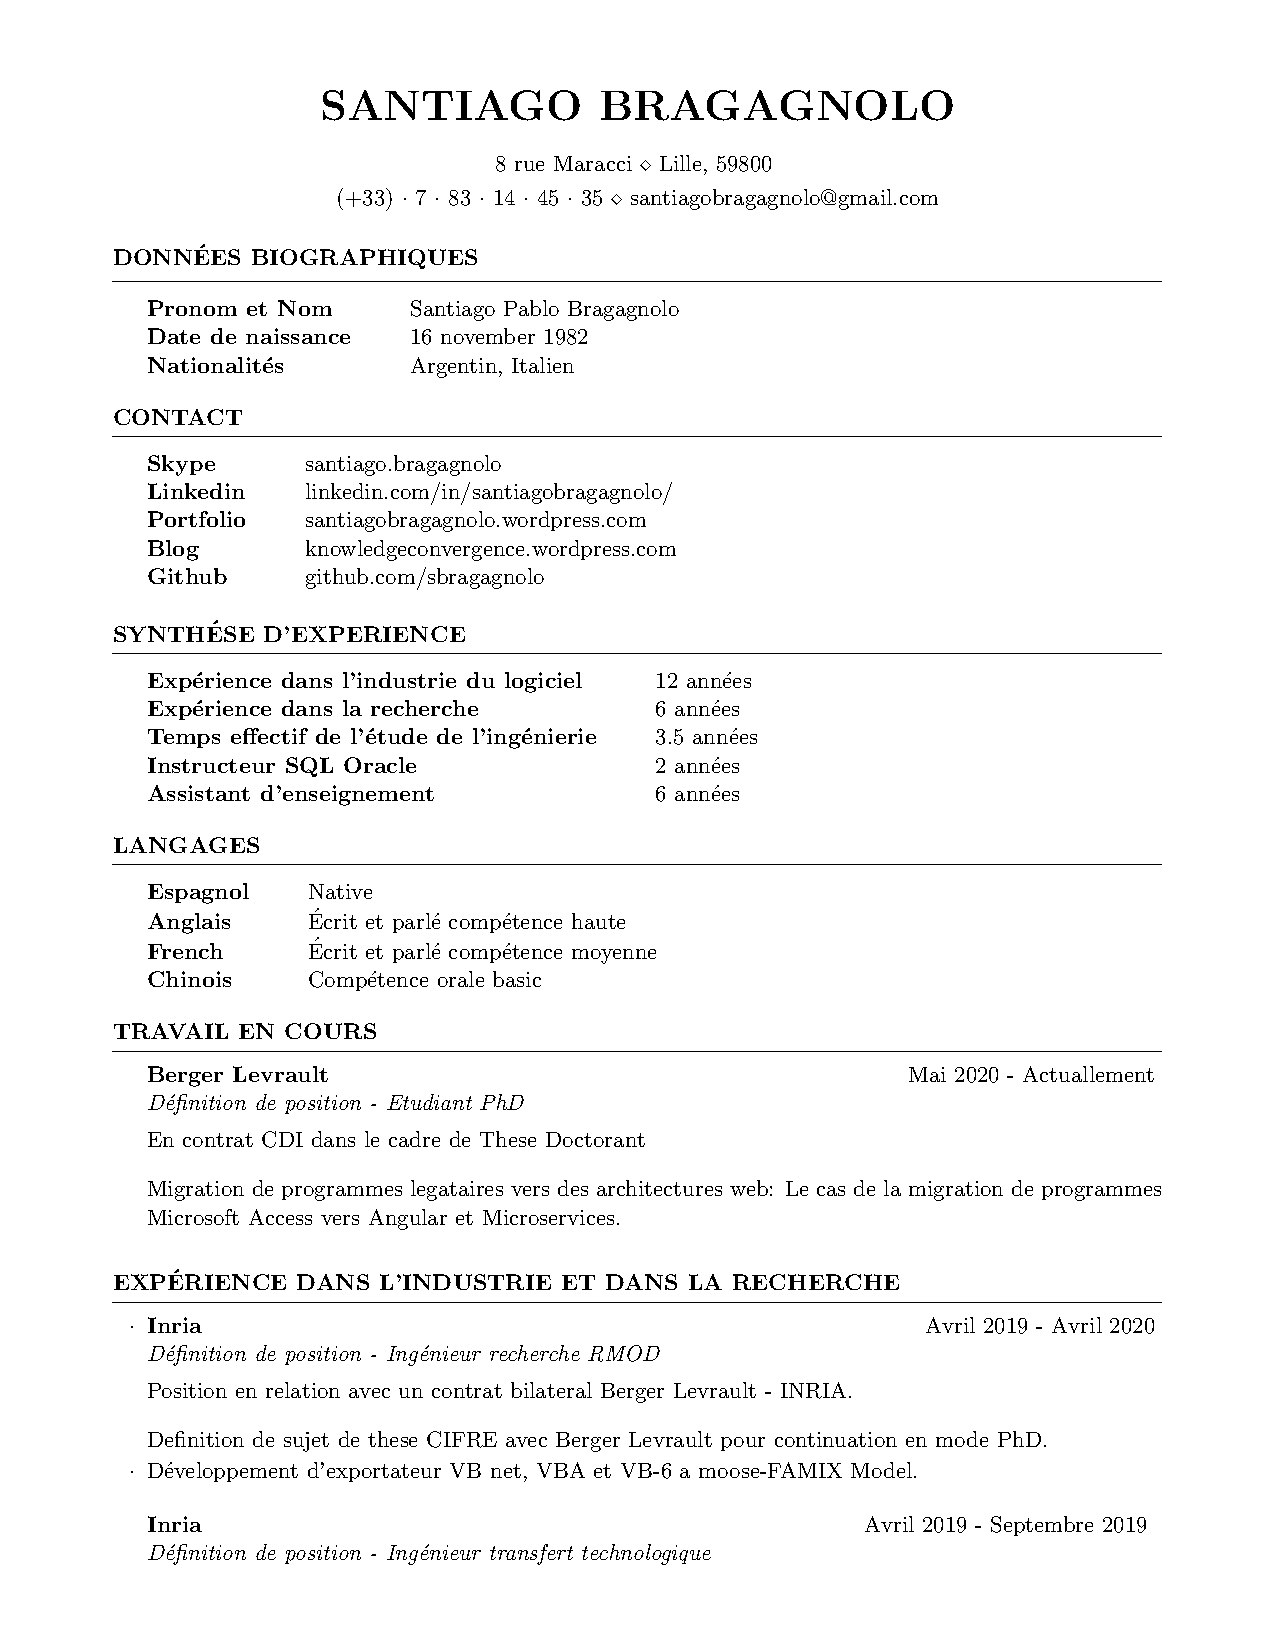
\includepdf[pages=-]{docs/Doc2-CV.pdf}

\section{Passeport}
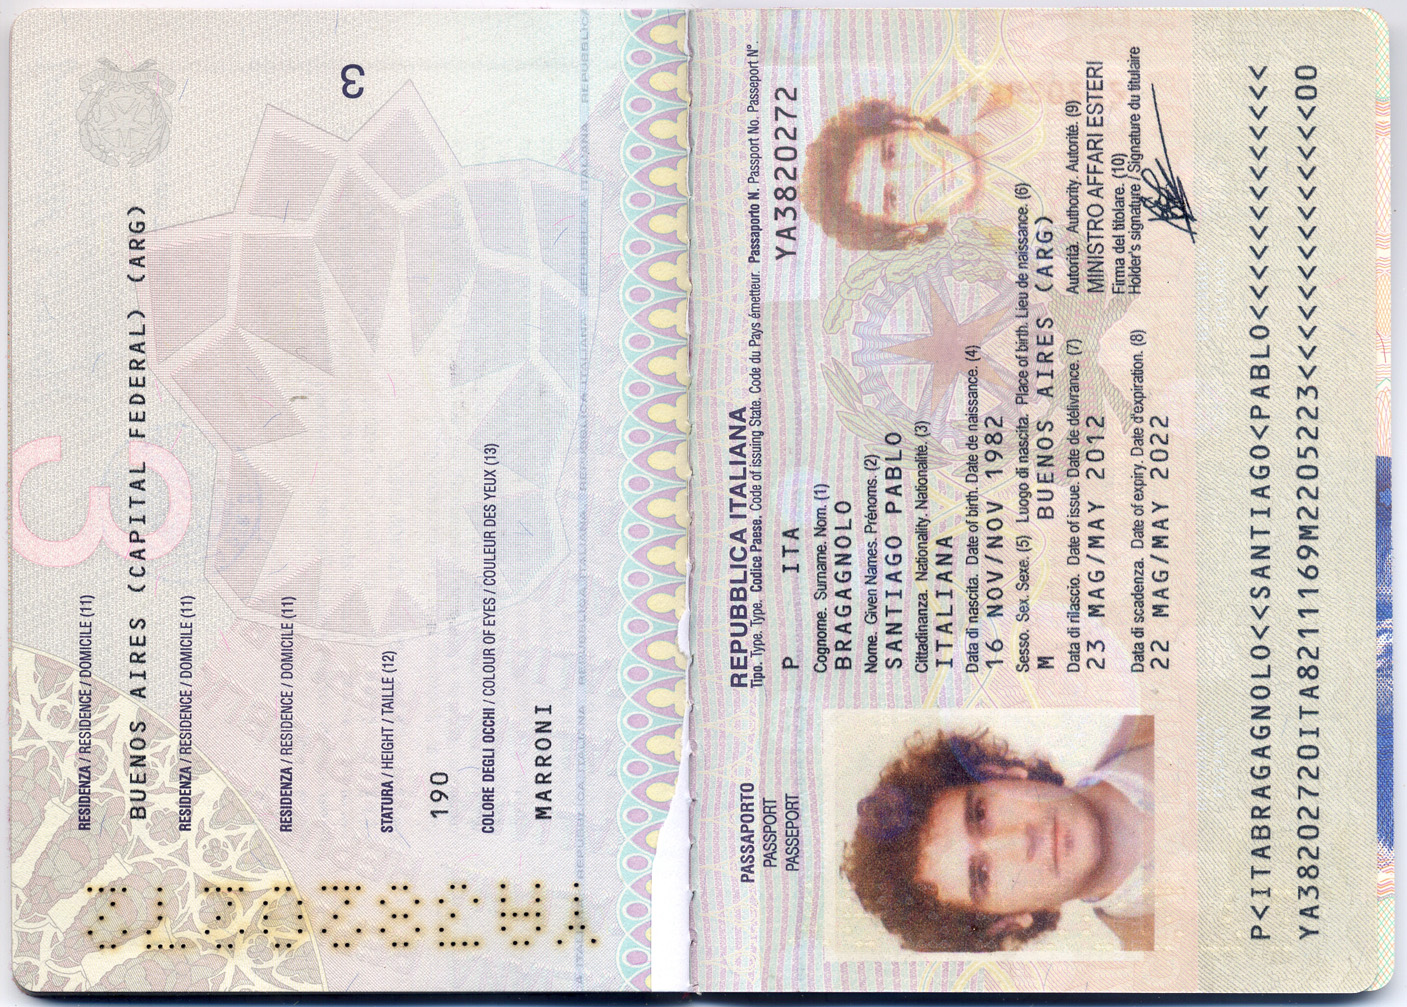
\includegraphics[width=15cm,height=15cm,keepaspectratio]{docs/Doc3-Passport.jpg}

\section {Notes Obtenus}
    Mon titre de Master a été obtenu a travers un processus de Validation des Acquis de l'Experience (VAE). Pour ce motive je ne peux pas offrir les notes et programmes. 
    Au lieu de ce documents, je rajoute une copie du certificat de la VAE. 
    
 
\includegraphics[width=15cm,height=15cm,keepaspectratio]{docs/Doc4-VAE.jpeg}   
  
\section{Diploma} 

 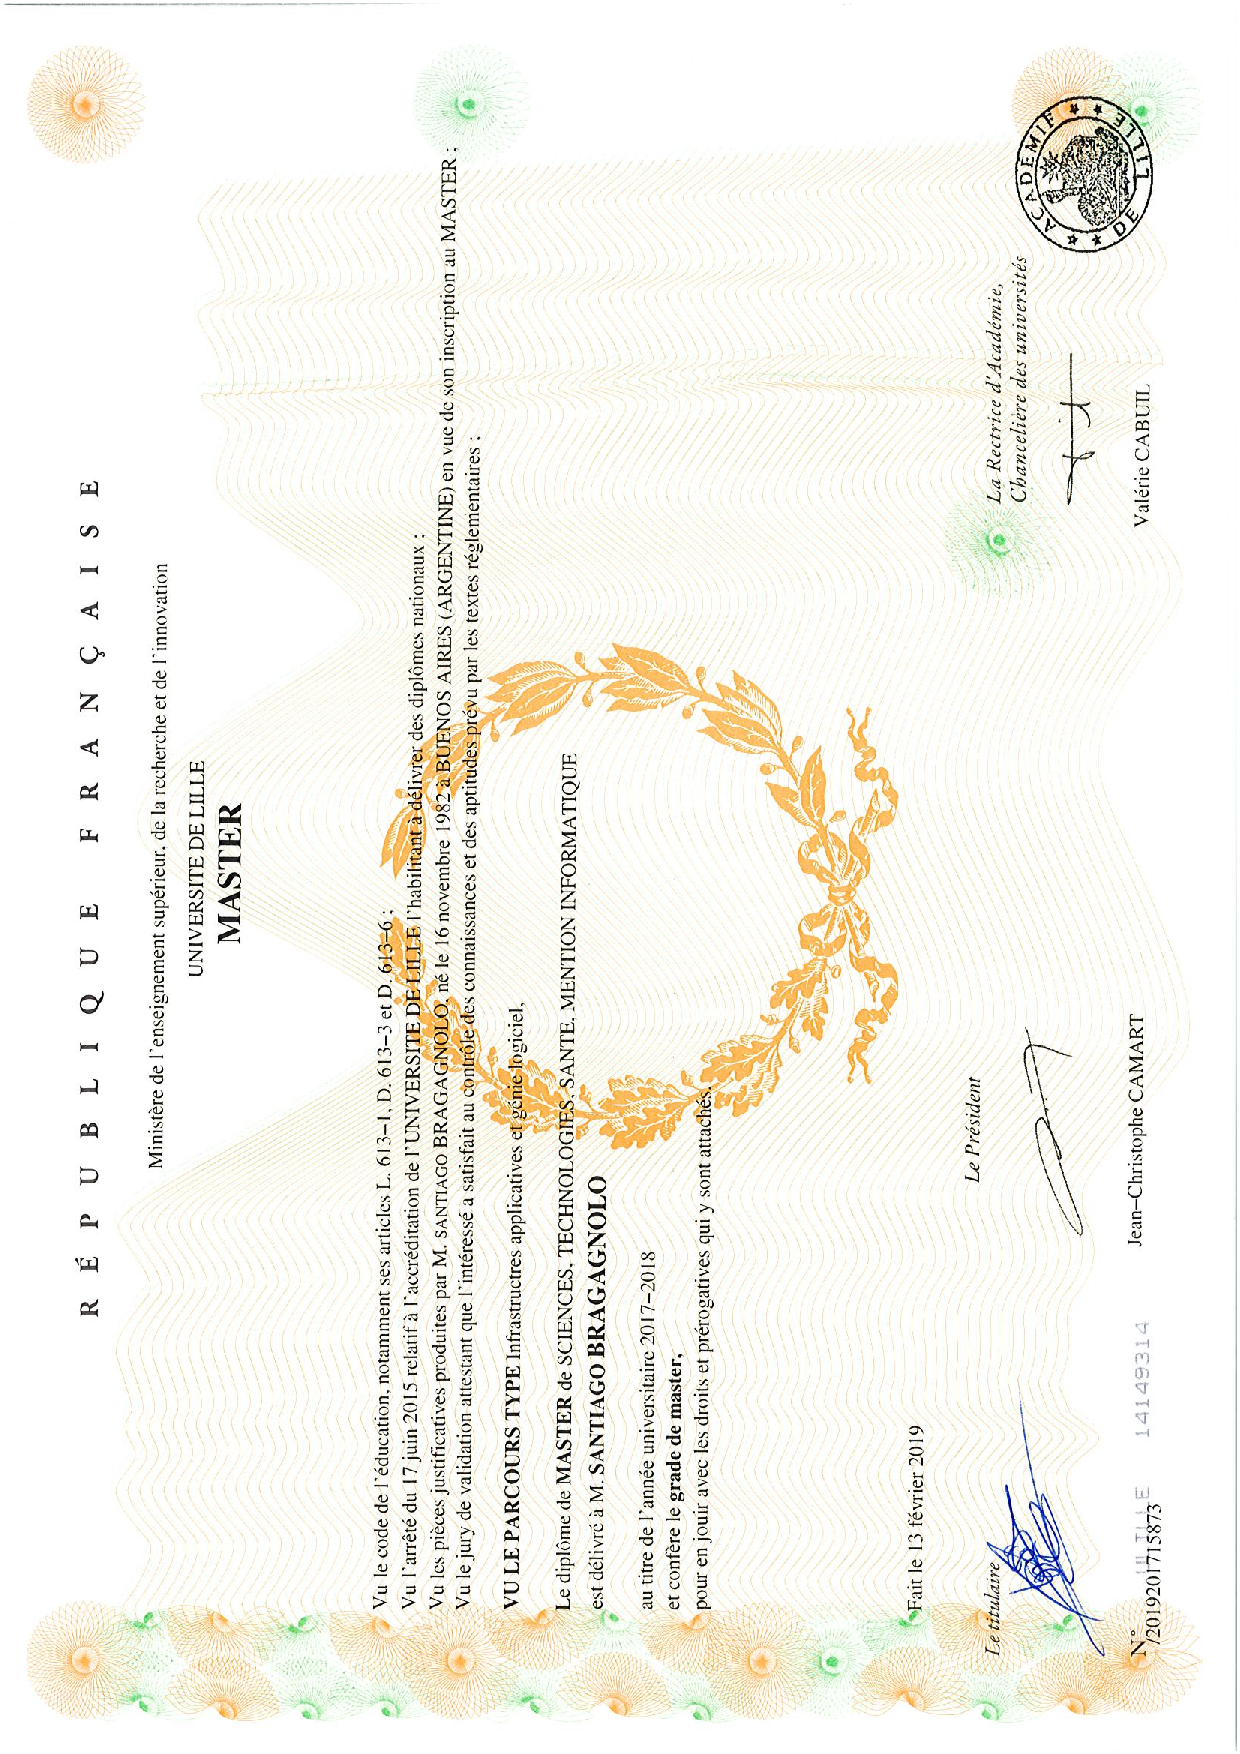
\includegraphics[width=15cm,height=15cm,keepaspectratio]{docs/Doc5-MasterSanti.pdf}   


\section{Travaux personnels}
   Ici je rajoute trois articles ou je suis le author principal, un quatrieme ou je suis le deuxième author.
 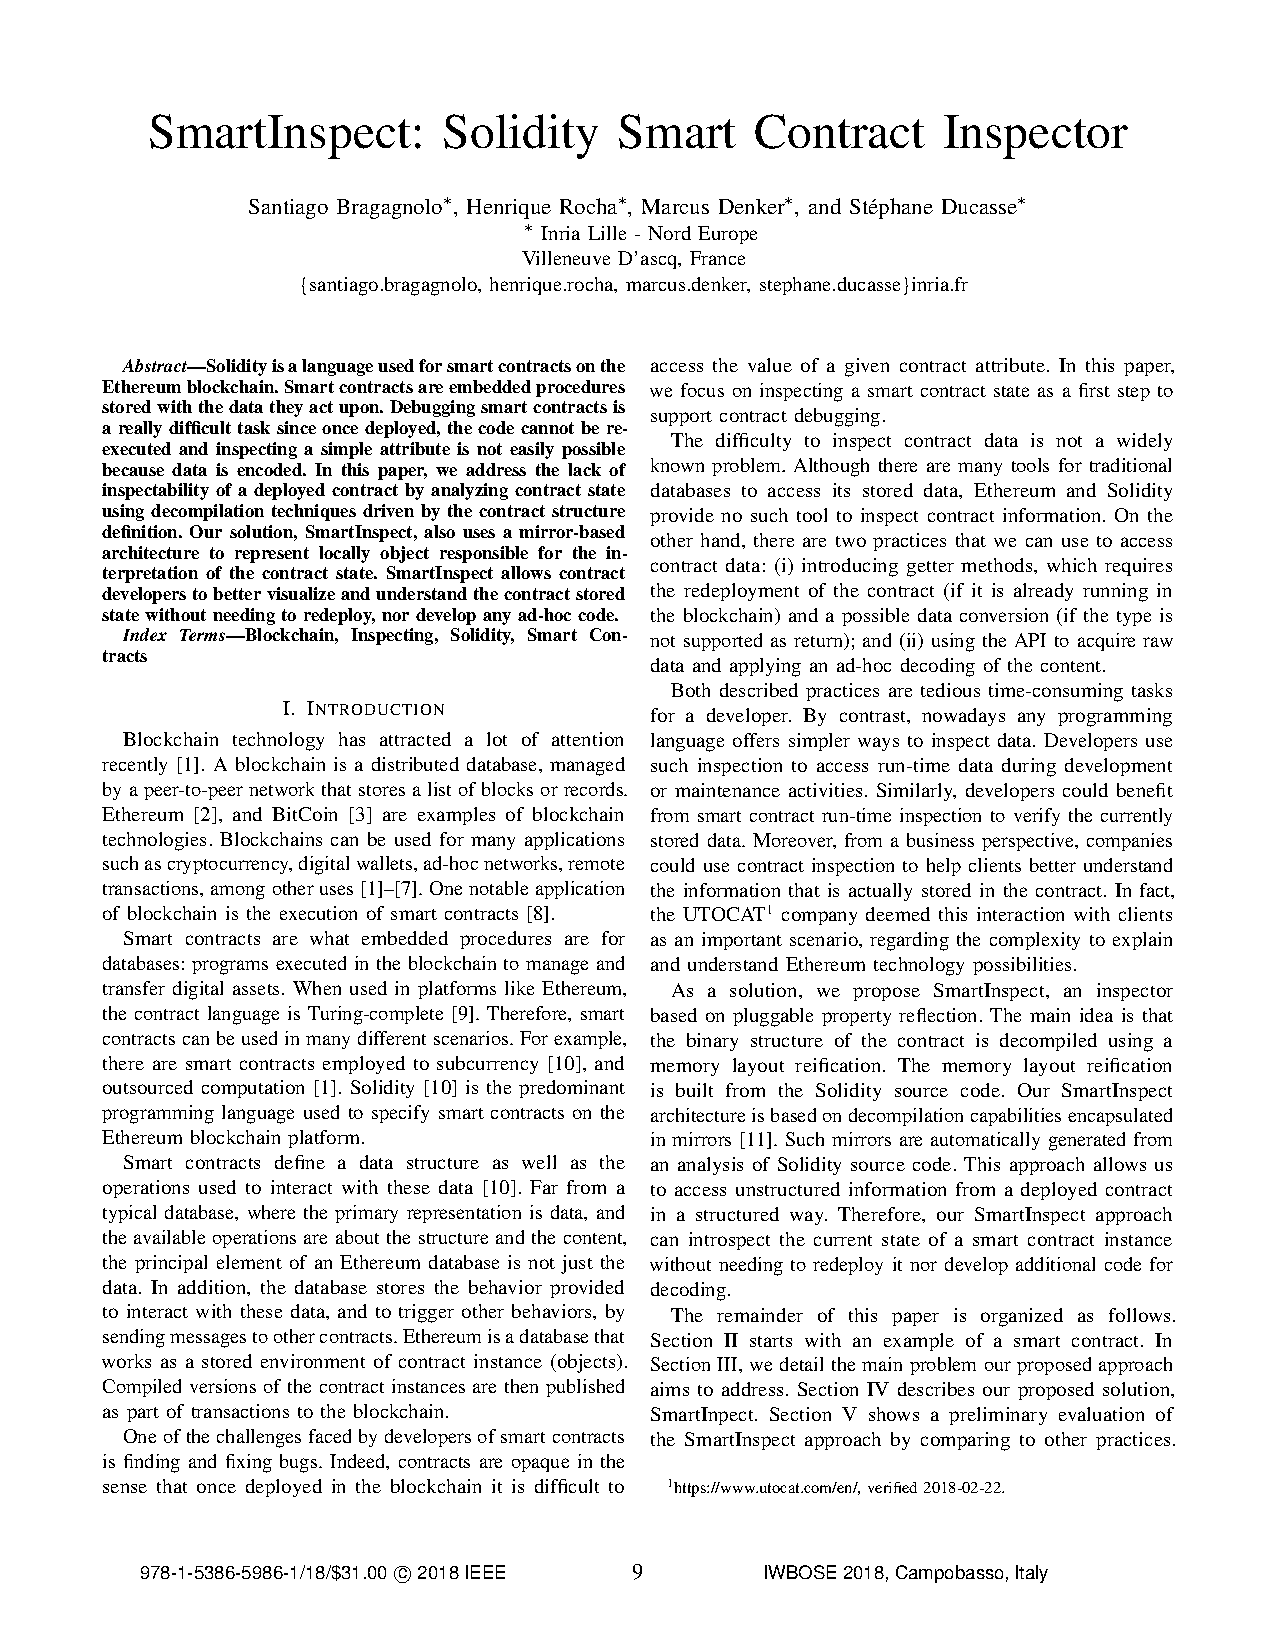
\includepdf[pages=-]{docs/Doc6-Paper1.pdf}
 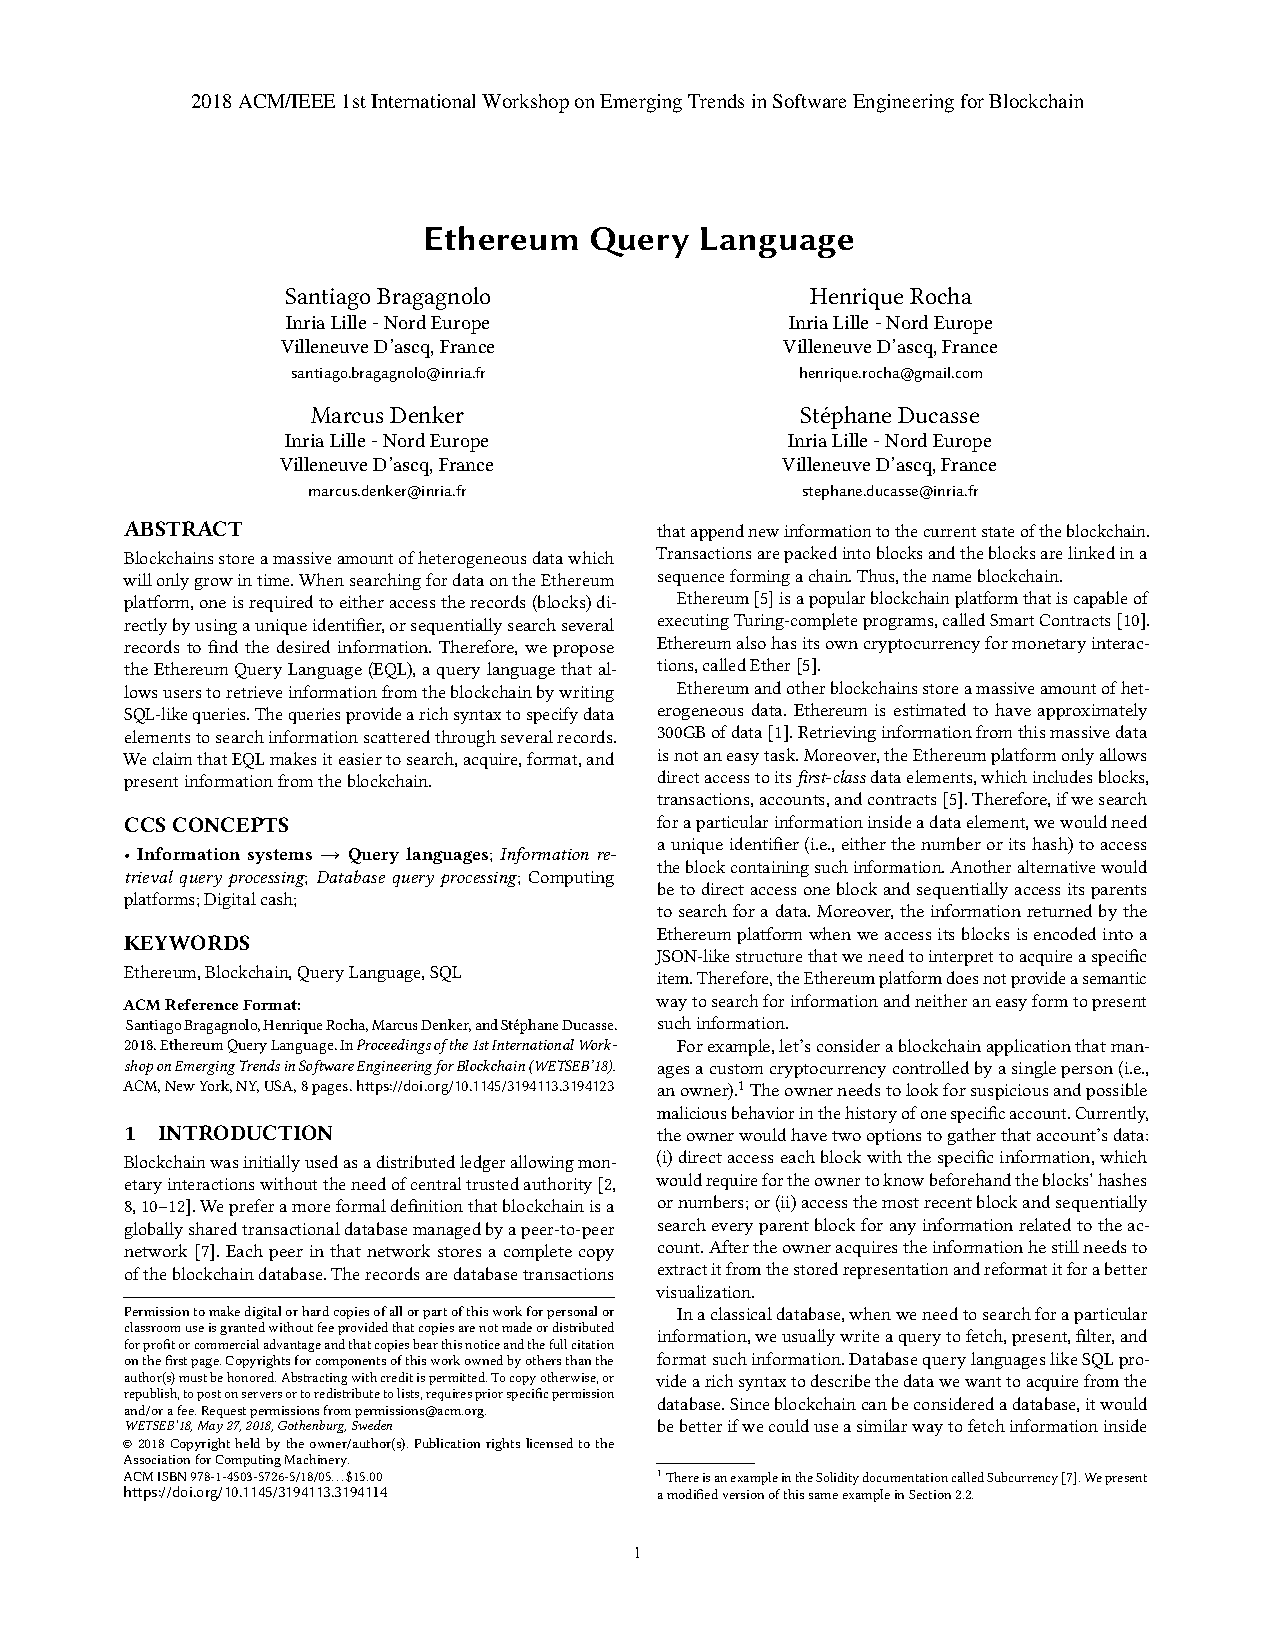
\includepdf[pages=-]{docs/Doc7-Paper2.pdf}
 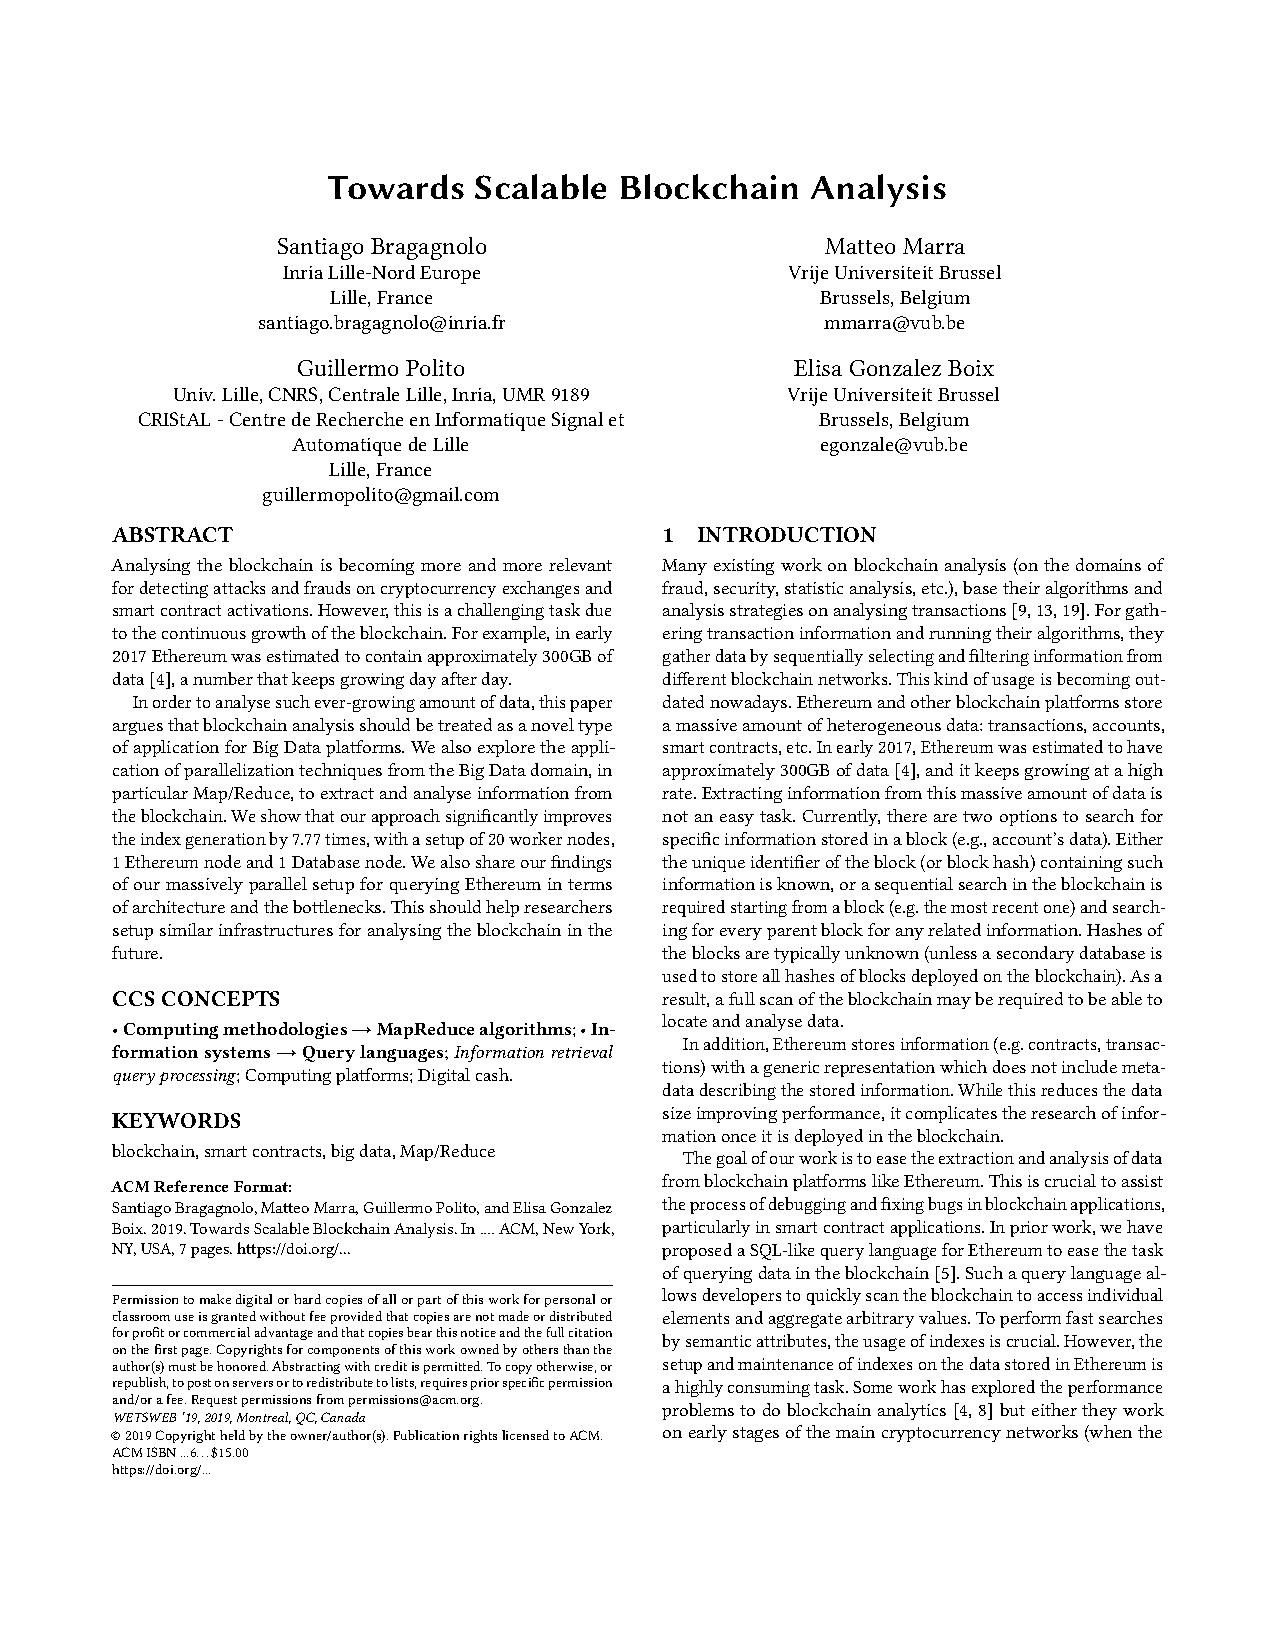
\includepdf[pages=-]{docs/Doc8-Paper3.pdf}
 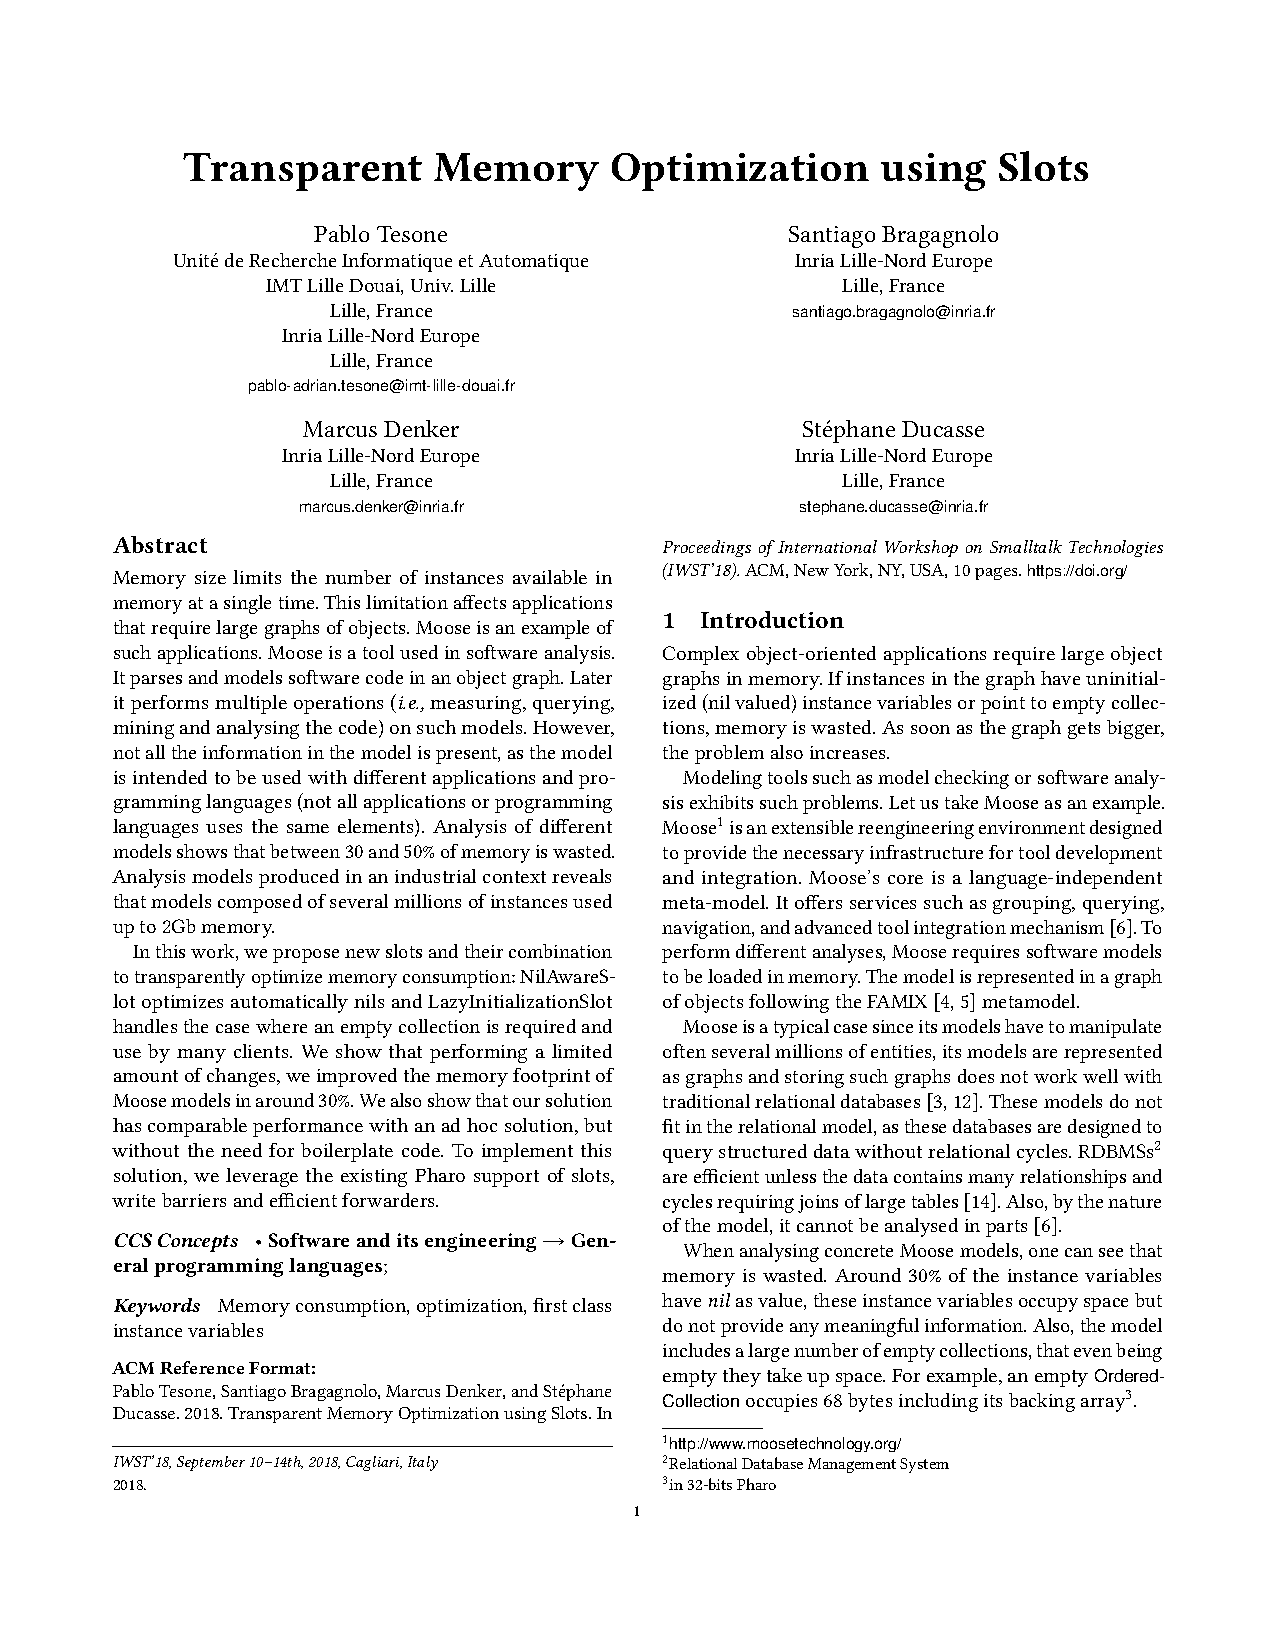
\includepdf[pages=-]{docs/Doc9-Paper4.pdf}
 

\section{Lettres de recommandation}

 
\includepdf[pages=-]{docs/Doc10-lettre_recommandation_Santiago_Bragagnolo.pdf}
 
\includepdf[pages=-]{docs/Doc10-RecomBragagnoloCIFRE-ANRT.pdf}


\section{Lettre de recommandation du directeur de recherche}
 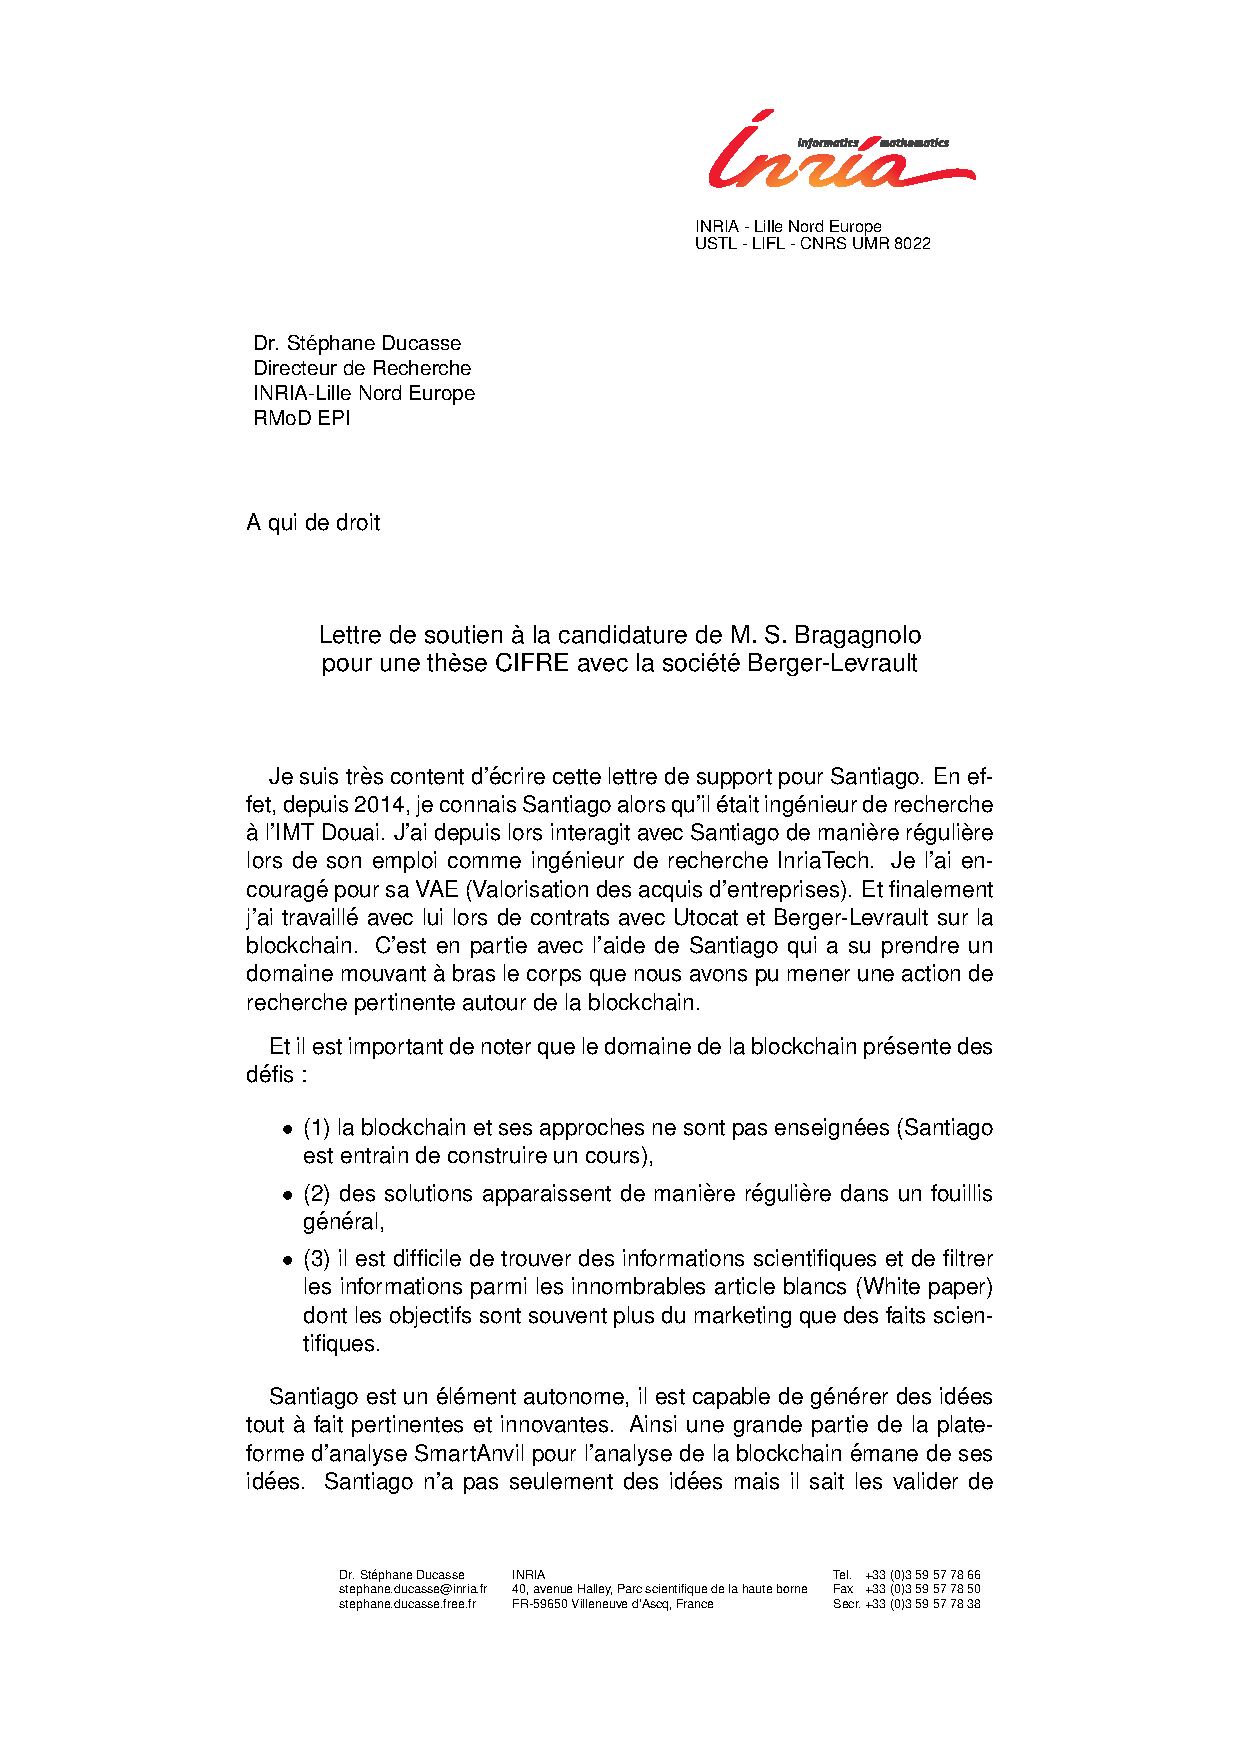
\includepdf[pages=-]{docs/Doc11-DucassePourBragagnoloPhD.pdf}
 
 
 
\section{Attestation de financement}
  Je suis déjà employé par Berger Levrault en mode CDI, dans le cadre de recherche pour cet these. Le contrat n'est pas encore signé a cause du confinement du a Covid-19. 
  A la place du contrat je laisse ici la lettre d'engagement signée au moment de la demande a l'ANRT. 
  
  

 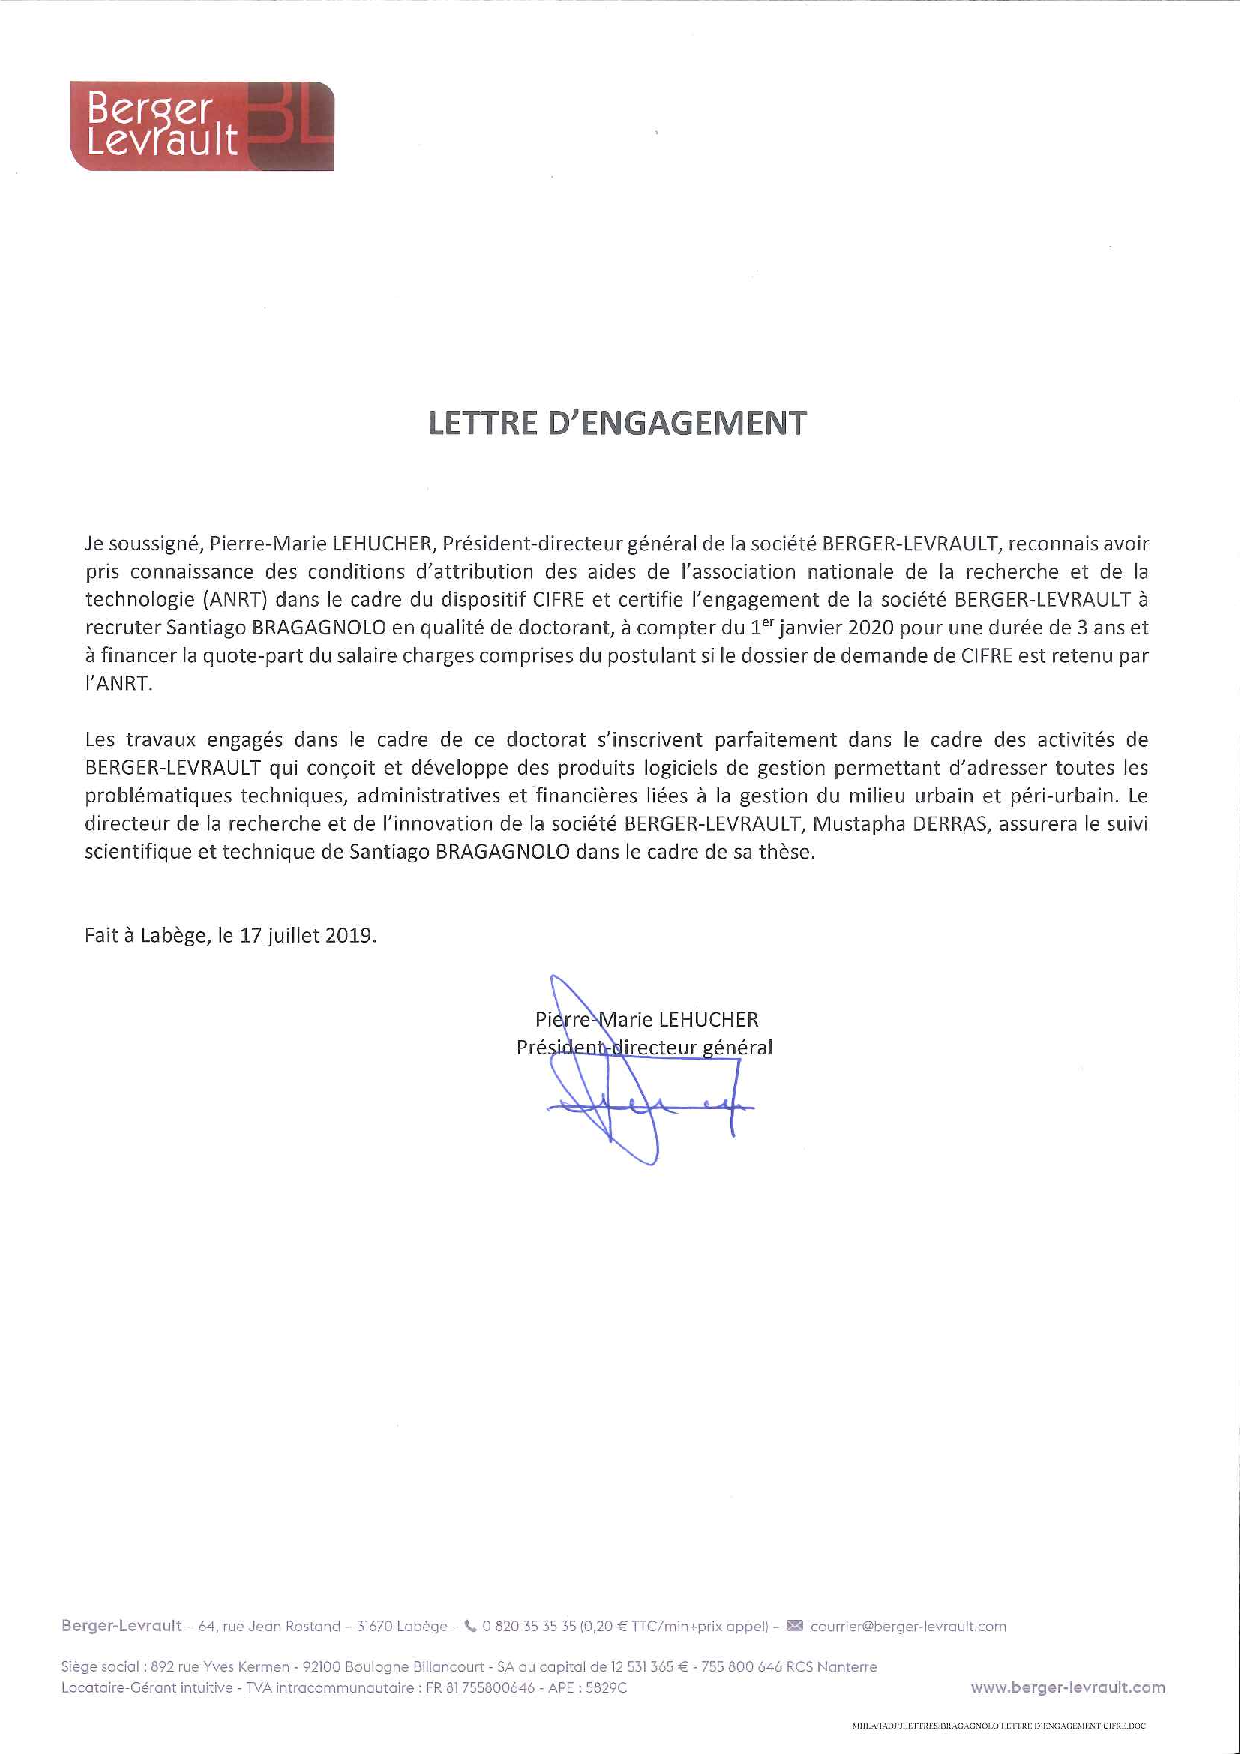
\includepdf[pages=-]{docs/Doc12-Lettre-Engagement-BL.pdf}


%----------------------------------------------------------------------------------------

\end{document}







